\documentclass[paper=a4, fontsize=11pt]{article}

%----------------------------------------------------------------------------------------
%	PACKAGES AND OTHER DOCUMENT CONFIGURATIONS
%----------------------------------------------------------------------------------------

\usepackage{amsmath,amsfonts,amsthm} % Math packages
\usepackage{sectsty} % Allows customizing section commands
\allsectionsfont{\centering \normalfont\scshape} % Make all sections centered, the default font and small caps

\usepackage{fancyhdr} % Custom headers and footers
\pagestyle{fancyplain} % Makes all pages in the document conform to the custom headers and footers
\fancyhead{} % No page header - if you want one, create it in the same way as the footers below
\fancyfoot[L]{} % Empty left footer
\fancyfoot[C]{} % Empty center footer
\fancyfoot[R]{\thepage} % Page numbering for right footer
\renewcommand{\headrulewidth}{0pt} % Remove header underlines
\renewcommand{\footrulewidth}{0pt} % Remove footer underlines
\setlength{\headheight}{13.6pt} % Customize the height of the header

\numberwithin{equation}{section} % Number equations within sections (i.e. 1.1, 1.2, 2.1, 2.2 instead of 1, 2, 3, 4)
\numberwithin{figure}{section} % Number figures within sections (i.e. 1.1, 1.2, 2.1, 2.2 instead of 1, 2, 3, 4)
\numberwithin{table}{section} % Number tables within sections (i.e. 1.1, 1.2, 2.1, 2.2 instead of 1, 2, 3, 4)

%\setlength\parindent{0pt} % Removes all indentation from paragraphs - comment this line for an assignment with lots of text
\setlength{\parskip}{1em}
\renewcommand{\baselinestretch}{1.5}

\usepackage{tikz-qtree}
\usepackage{lscape}

\usepackage{graphicx}
\graphicspath{ {images/} }

\usepackage{xepersian}
\settextfont[Path=fonts/]{Vazir.ttf}
%\setlatintextfont{Times New Roman}

%----------------------------------------------------------------------------------------
%	TITLE SECTION
%----------------------------------------------------------------------------------------

\newcommand{\horrule}[1]{\rule{\linewidth}{#1}} % Create horizontal rule command with 1 argument of height

\title{
\normalfont\normalsize

\includegraphics[scale=0.1]{aut}
\hspace{5cm}

\includegraphics[scale=0.1]{ceit} \\
\textsc دانشگاه صنعتی امیرکبیر \\
\textsc دانشکده مهندسی کامپیوتر و فناوری اطلاعات
\horrule{0.5pt} \\ [0.4cm] % Thin top horizontal rule
\huge معماری سوئیچ و روترهای با کارآیی بالا \\ % The assignment title
\huge تمرین دوم \\ % The assignment title
\horrule{2pt} \\ [0.5cm] % Thick bottom horizontal rule
}

\author{پرهام الوانی}

\date{\normalsize\today} % Today's date or a custom date

\begin{document}

\maketitle % Print the title

\section{سوال اول}

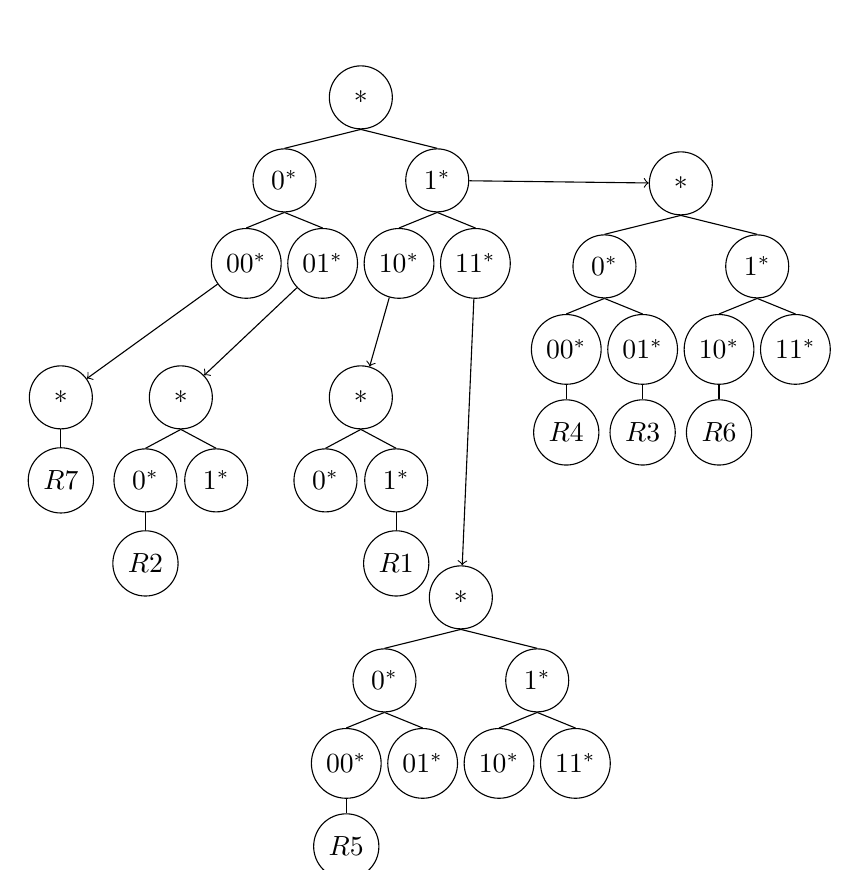
\begin{tikzpicture}[every tree node/.style={draw, circle, minimum width=0.8cm}]
    \Tree
    [.$*$
        % 0
        [.$0^*$
            \node(00){$00^*$};
            \node(01){$01^*$};
        ]
        % 1
        [. \node(1){$1^*$};
            \node(10){$10^*$};
            \node(11){$11^*$};
        ]
    ]
    \begin{scope}[shift={(-1.5in,-1.5in)}]
        \Tree
        [. \node(r00){$*$};
            [. $R7$ ]
        ]
    \end{scope}
    \begin{scope}[shift={(-0.9in,-1.5in)}]
        \Tree
        [. \node(r01){$*$};
            [. $0^*$
                [. $R2$ ]
            ]
            [. $1^*$
            ]
        ]
    \end{scope}
    \begin{scope}[shift={(1.6in,-0.43in)}]
        \Tree
        [. \node(r1){$*$};
            [. $0^*$
                [. $00^*$ [. $R4$ ] ]
                [. $01^*$ [. $R3$ ] ]
            ]
            [. $1^*$
                [. $10^*$ [. $R6$ ] ]
                [. $11^*$ ]
            ]
        ]
    \end{scope}
    \begin{scope}[shift={(0in,-1.5in)}]
        \Tree
        [. \node(r10){$*$};
            [. $0^*$
            ]
            [. $1^*$
                [. $R1$ ]
            ]
        ]
    \end{scope}
    \begin{scope}[shift={(0.5in,-2.5in)}]
        \Tree
        [. \node(r11){$*$};
            [. $0^*$
                [. $00^*$ [. $R5$ ] ]
                [. $01^*$ ]
            ]
            [. $1^*$
                [. $10^*$ ]
                [. $11^*$ ]
            ]
        ]
    \end{scope}



    \draw[->] (00)--(r00);
    \draw[->] (1)--(r1);
    \draw[->] (01)--(r01);
    \draw[->] (10)--(r10);
    \draw[->] (11)--(r11);
\end{tikzpicture}

\section{سوال دوم}

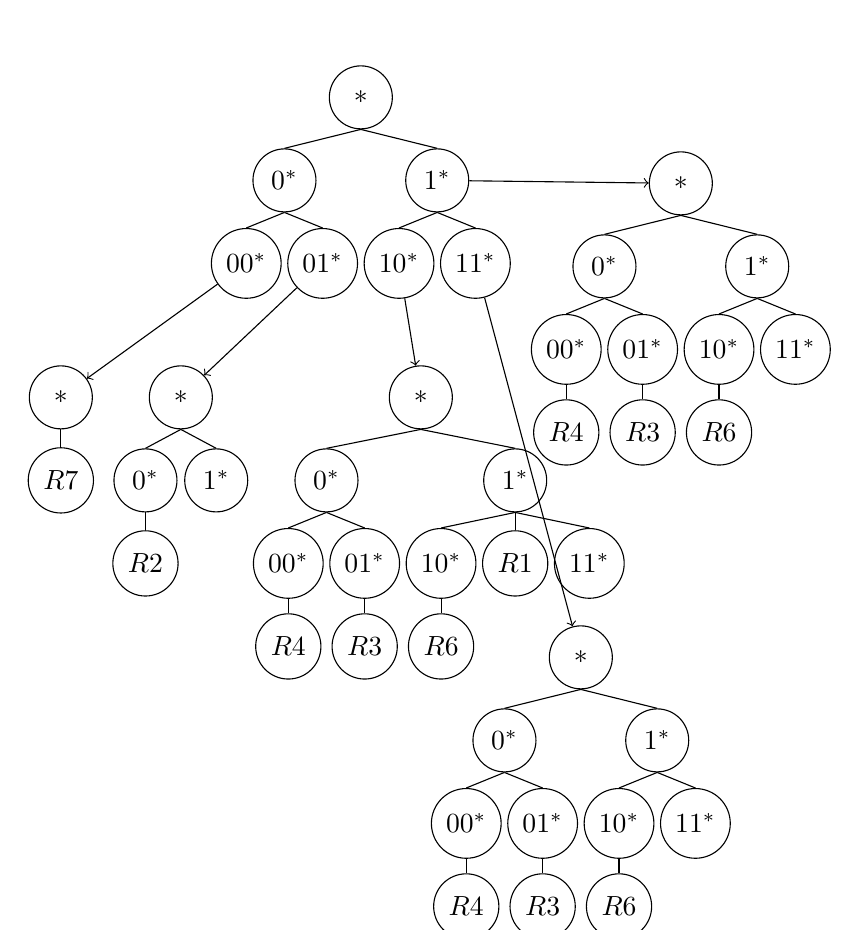
\begin{tikzpicture}[every tree node/.style={draw, circle, minimum width=0.8cm}]
    \Tree
    [.$*$
        % 0
        [.$0^*$
            \node(00){$00^*$};
            \node(01){$01^*$};
        ]
        % 1
        [. \node(1){$1^*$};
            \node(10){$10^*$};
            \node(11){$11^*$};
        ]
    ]
    \begin{scope}[shift={(-1.5in,-1.5in)}]
        \Tree
        [. \node(r00){$*$};
            [. $R7$ ]
        ]
    \end{scope}
    \begin{scope}[shift={(-0.9in,-1.5in)}]
        \Tree
        [. \node(r01){$*$};
            [. $0^*$
                [. $R2$ ]
            ]
            [. $1^*$
            ]
        ]
    \end{scope}
    \begin{scope}[shift={(1.6in,-0.43in)}]
        \Tree
        [. \node(r1){$*$};
            [. $0^*$
                [. $00^*$ [. $R4$ ] ]
                [. $01^*$ [. $R3$ ] ]
            ]
            [. $1^*$
                [. $10^*$ [. $R6$ ] ]
                [. $11^*$ ]
            ]
        ]
    \end{scope}
    \begin{scope}[shift={(0.3in,-1.5in)}]
        \Tree
        [. \node(r10){$*$};
            [. $0^*$
                [. $00^*$ [. $R4$ ] ]
                [. $01^*$ [. $R3$ ] ]
            ]
            [. $1^*$
                [. $10^*$ [. $R6$ ] ]
                [. $R1$ ]
                [. $11^*$ ]
            ]
        ]
    \end{scope}
    \begin{scope}[shift={(1.1in,-2.8in)}]
        \Tree
        [. \node(r11){$*$};
            [. $0^*$
                [. $00^*$ [. $R4$ ] ]
                [. $01^*$ [. $R3$ ] ]
            ]
            [. $1^*$
                [. $10^*$ [. $R6$ ] ]
                [. $11^*$ ]
            ]
        ]
    \end{scope}



    \draw[->] (00)--(r00);
    \draw[->] (1)--(r1);
    \draw[->] (01)--(r01);
    \draw[->] (10)--(r10);
    \draw[->] (11)--(r11);
\end{tikzpicture}


\end{document}